\section{Análise Financeira}

Esta seção apresenta a avaliação econômica do projeto, considerando diferentes cenários de receita e custos operacionais.  
O objetivo é demonstrar a viabilidade financeira do sistema quando estruturado como um modelo \gls{saas}, destacando a relação entre investimentos, receitas projetadas e retorno esperado.  
A análise contempla tanto a perspectiva conservadora quanto cenários mais otimistas, fornecendo uma visão abrangente sobre a sustentabilidade econômica do projeto e os fatores que influenciam o sucesso financeiro da aplicação.

\subsection{Cenários}

Nesta subseção, são detalhados três cenários de desempenho financeiro do projeto: pessimista, realista e otimista.  
Cada cenário considera diferentes taxas de crescimento da base de clientes e respectivas receitas provenientes das mensalidades, bem como os custos associados à manutenção e operação do sistema.  
A análise permite identificar o ponto de equilíbrio, projetar lucros ou prejuízos e avaliar indicadores financeiros importantes, como ROI e Payback Period, para cada contexto estudado.


\subsubsection{Cenário Realista}

A Figura \ref{fig:cenario-realista} apresenta as receitas e custos acumulados no cenário realista considerando o projeto como um \gls{saas}. Nesse contexto, para o cálculo do acúmulo de receitas, estabeleceu-se um aumento mensal razoável de 15 clientes para o plano básico e 10 para o profissional.

Os custos consideram somente os gastos com mão de obra, infraestrutura e mensalidades ou licenças das ferramentas utilizadas no desenvolvimento e manutenção da aplicação.

No cenário realista, o ponto de equilíbrio é atingido no sétimo mês e, ao fim dos doze meses de análise, há um lucro de R\$ 66 mil.

\begin{figure}[h]
	\centering
	\caption{Cenário realista}
	\fbox{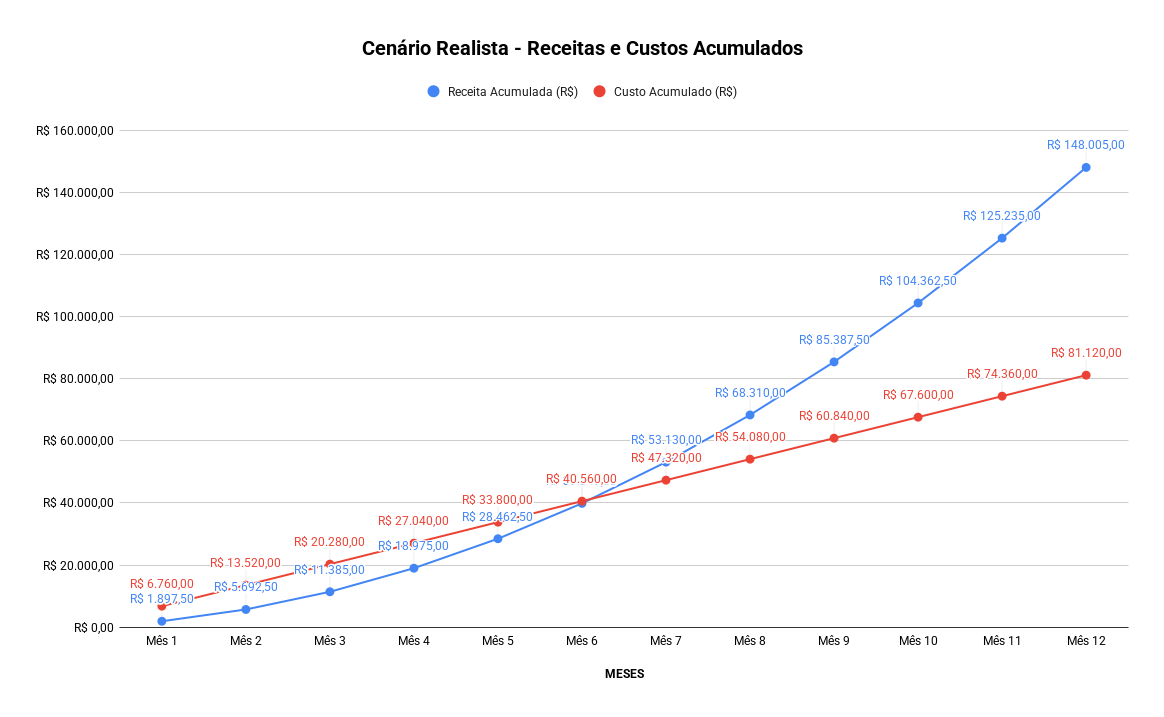
\includegraphics[width=0.9\textwidth]{cap05-viabilidade/imagens/cenario-realista.png}}
	\label{fig:cenario-realista}
	\fonte{Produzido pelos autores}
\end{figure}
\subsubsection{Cenário otimista}

A Figura \ref{fig:cenario-otimista} apresenta as receitas e custos acumulados no cenário otimista considerando o projeto como um \gls{saas}. Nesse contexto, para o cálculo do acúmulo de receitas, estabeleceu-se um aumento mensal acentuado de 30 clientes para o plano básico e 25 para o profissional.

Os custos consideram somente os gastos com mão de obra, infraestrutura e mensalidades ou licenças das ferramentas utilizadas no desenvolvimento e manutenção da aplicação.

No cenário otimista, o ponto de equilíbrio é atingido no terceiro mês e, ao fim dos doze meses de análise, há um lucro de R\$ 253 mil.

\begin{figure}[h]
	\centering
	\caption{Cenário otimista}
	\fbox{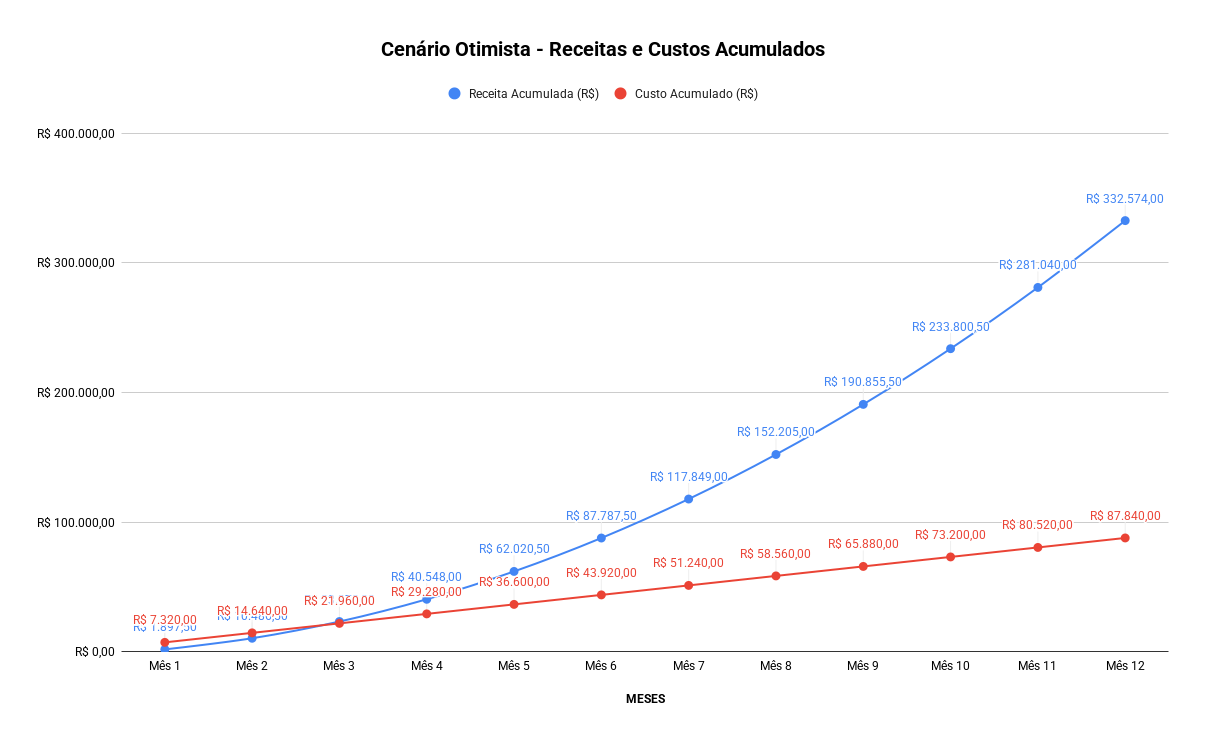
\includegraphics[width=0.9\textwidth]{cap05-viabilidade/imagens/cenario-otimista.png}}
	\label{fig:cenario-otimista}
	\fonte{Produzido pelos autores}
\end{figure}
\subsubsection{Cenário pessimista}

A Figura \ref{fig:cenario-pessimista} apresenta as receitas e custos acumulados no cenário pessimista considerando o projeto como um \gls{saas}. Nesse contexto, para o cálculo do acúmulo de receitas, estabeleceu-se um aumento mensal baixo de 5 clientes para o plano básico e 3 para o profissional.

Os custos consideram somente os gastos com mão de obra, infraestrutura e mensalidades ou licenças das ferramentas utilizadas no desenvolvimento e manutenção da aplicação.

No cenário pessismista, o ponto de equilíbrio não é atingido no doze meses de análise e, ao fim desse intervalo de tempo, há um prejuízo de R\$ 34 mil.
\begin{figure}[h]
	\centering
	\caption{Cenário pessimista}
	\fbox{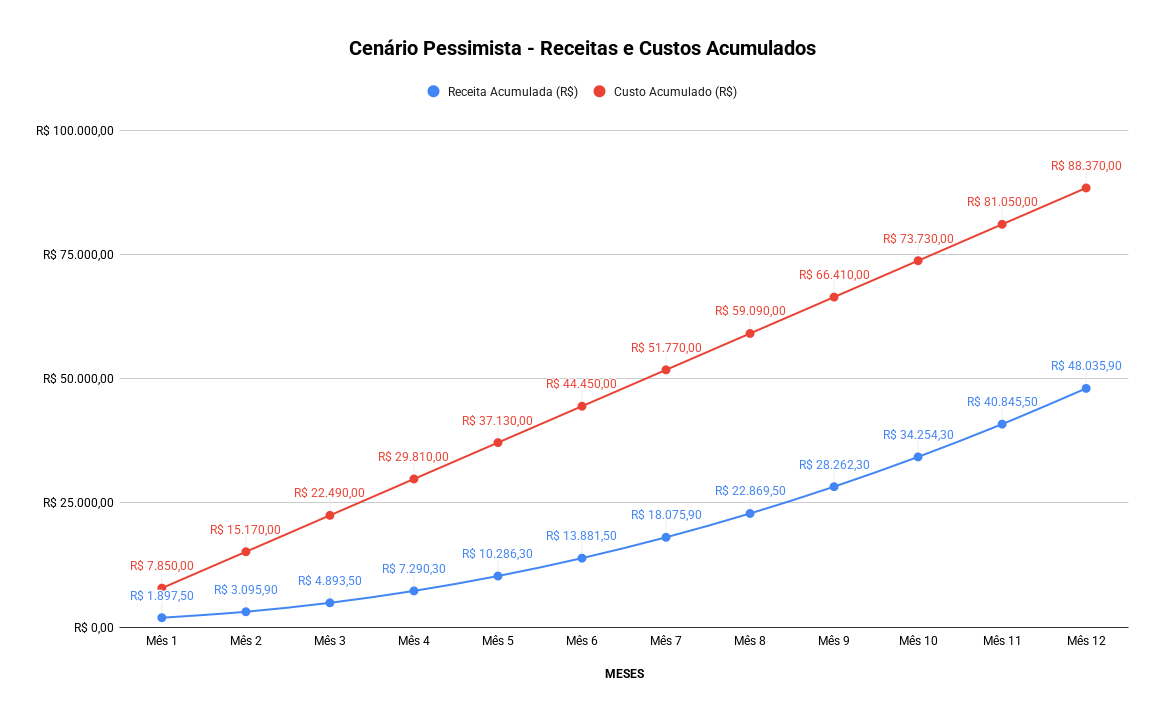
\includegraphics[width=0.9\textwidth]{cap05-viabilidade/imagens/cenario-pessimista.png}}
	\label{fig:cenario-pessimista}
	\fonte{Produzido pelos autores}
\end{figure}

\subsection{Indicadores financeiros}

Para complementar a análise dos cenários apresentados, foram utilizadas métricas financeiras amplamente empregadas em estudos de viabilidade econômica, como o \textbf{Retorno sobre o Investimento (ROI)} e o \textbf{Período de Retorno (Payback Period)}.

O \textbf{ROI (Return on Investment)} mede a relação entre o lucro obtido e o investimento inicial, indicando o percentual de retorno gerado pelo projeto. Sua fórmula é:

\[
ROI = \frac{\text{Lucro Líquido}}{\text{Investimento Total}} \times 100
\]

O \textbf{Payback Period} representa o tempo necessário para recuperar o investimento inicial a partir das receitas acumuladas, sendo calculado como:

\[
\text{Payback} = \frac{\text{Investimento Inicial}}{\text{Receita Líquida Média Mensal}}
\]

\subsubsection{Cenário realista}

Considerando o cenário realista, em que o aumento mensal é de 15 clientes no plano básico e 10 no profissional, ao fim de 12 meses, o lucro acumulado obtido somente pelas mensalidades é de aproximadamente R\$ 59 mil.  
Com investimento inicial de R\$ 60.840 (Tabela \ref{tab:custo-total-projeto}), o ROI estimado é de cerca de 108\% e o \textit{payback} ocorre antes de completar um ano.

\subsubsection{Cenário otimista}

No cenário otimista, com crescimento de 30 clientes no básico e 25 no profissional por mês, ao fim de 12 meses, o lucro acumulado pelas mensalidades é de R\$ 253 mil, resultando em ROI de aproximadamente 416\% e confirmando o rápido retorno do investimento. O \textit{payback} ocorre em cerca de 3 meses.

\subsubsection{Cenário pessimista}

No cenário pessimista, com aumento de apenas 5 clientes no plano básico e 3 no profissional por mês, ao fim de 12 meses, o projeto apresenta prejuízo de R\$ 34 mil, refletindo ROI negativo e ausência de payback no período analisado.
